\section{Design of C-=-1}
\label{language-design}

C-=-1 was designed as a compiled, low-level, non-garbage-collected programming language, similar to C, C++ or Rust.
What diffirentiates C-=-1 are its two founding principles: all code is executable at compile-time and support rich metaprogramming.
The primary purpose of the language was to research how these ideas influence software written in it \cite{grabski2022compilation}.

\subsection{Type system}

\subsection{Attributes and metaprogramming}

\section{Design of the compiler}
\label{compiler-design}

CTFE First apporach was created during implementation of the first compiler for the C-=-1 language\cite{grabski2022compilation}.
CTFE First compiler has four major components: Frontend, Interpreter, Compiler Interface and Backend.
Figure \ref{CTFE-first-compiler-structure} contains a diagram with an overview of how these pieces interact with eachother, during the compilaton process.
Frontend, described in chapter \ref{frontend}, parses the code in the compiled language and constructs its intermidaite representation, using interpreter's data structures.
It is used to analyze both user code and the Compiler Interface.
After the intermidiate representation is constructed, it is passed on to the Interpreter, which was described in chapter \ref{interpreter}.
Compiler Interface intermidiate representation is then executed, using the user program as data. 
This step converts the semantic model of the program into the backends intermidiate language.
This process has been further explained in chapter \ref{compiler-interface}.
Finaly the Backend generates the executable file.

\begin{figure}
	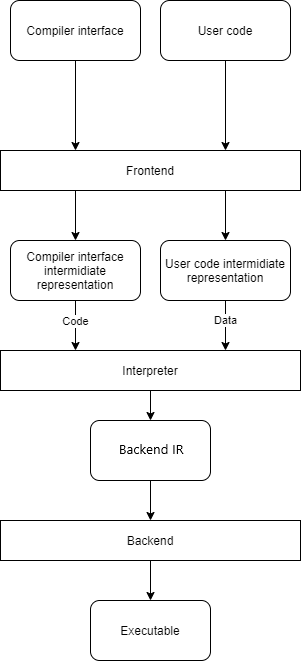
\includegraphics[height=10cm]{pictures/compiler-structure.png}
	\caption{CTFE First compiler structure}
	\label{CTFE-first-compiler-structure}
\end{figure}

\subsection{Frontend}
\label{frontend}

In the CTFE First approach, frontend serves the same role of constructing the programs intermidiate representation, as in conventional compilers \cite{puntambekar:compiler_design}.
The major difference lays in the data structures used to represent the program.

\subsection{Interpreter}
\label{interpreter}

\subsection{Compiler interface} 
\label{compiler-interface}

\subsection{Backend}
\label{backend}

CTFE First does not put any additional requierments on compiler backend.
When using this pattern, an out-of-the-box backend library, can be used, as was the case with C-=-1 compiler.

The backend code must be invokable from within the interpreted program in the target language.
Depending on how the interpreter was designed, this can represent a significant undertaking.
Compiler backends are large and for the Compiler Interface to take advantage of them fully, they must be fully available.
This means exposing each function and type within the library, to the interpreted code.
These bindings could feasibly be generated automatically \cite{marshalling_auto_generation}, but this tehnique was not used when implementing C-=-1 compiler.
